%% Thesis Template of GZ.Univ
%%   for using revised CASthesis package with LaTeX2e
%%
%% Created by snda.liu <thinksheng@foxmail.com>
%%
%% $Id: template.tex,v 0.33 2017/07/14 16:23:46   $

%%%请使用pdflatex或pdftexify编译






\documentclass[pdftex,notypeinfo,twoside,openany,UTF8,fntef]{CASthesis}
%oneside单面打印,twoside双面打印;支持环保,选择双面打印!
%twoside,openany只是表示pdf按照双面打印准备,当你去复印社时,依然需要跟老板说明:“你需要双面打印”。

\graphicspath{{chapter/}{figures/}} % 设置图形文件的搜索路径

\CTEXsetup[format+={\flushleft}]{section} % 小节标题靠左对齐

\allowdisplaybreaks[4] %公式强制分页

\renewcommand{\baselinestretch}{1.5} %行间距,默认为1.3
\usepackage{setspace}
\usepackage{booktabs}
\usepackage{graphicx}
\usepackage{times}
\usepackage{mathptmx}
\usepackage{subcaption}
\usepackage[]{algorithm2e}
\usepackage{booktabs}
\usepackage{relsize}
\usepackage{colortbl}
\usepackage{enumerate}
\usepackage{amsmath}
\usepackage{tikz}
\usepackage{pgf}
\usepackage{pbox}
\usepackage{rotating}
\usepackage{multirow}
\usepackage{balance}
\usepackage{tablefootnote}
\usepackage{epstopdf, epsfig}
\usepackage{url}
\usepackage{cleveref}[2012/02/15]
\usepackage{arydshln}
\usepackage[super]{gbt7714}
\usepackage{geometry} %设置页边距
\geometry{left=2.54cm,right=2.54cm,top=3.17cm,bottom=3.17cm}

\setcounter{tocdepth}{2}%设定目录层级(通常取值0-2之间)

\theoremstyle{THrm}{
	\newtheorem{question}{Question}[section]
	\newtheorem{property}{性质}[section]
	\newtheorem{assumption}{假设}[section]
	\newtheorem{claim}[lemma]{断言}
	
}


\begin{document}


%%%%%%%%%%%%%%%%%%%%%%%%%%%%%%
%% 封面部分
%%%%%%%%%%%%%%%%%%%%%%%%%%%%%%

  % 中文封面内容
 % \classification{TP309,TN918}%分类号
  %\confidential{公开}%密级
 % \serialnumber{2015010008}%论文编号
  \titlepage
  \newpage\thispagestyle{empty}
  
  
  \vspace*{10pt}
  \begin{center}
   	\heiti\zihao{-3}{\textbf{贵\ \ 州\ \ 大\ \ 学}}\\
   	\heiti\zihao{-3}{\textbf{2019届博士研究生学位论文}}\\
   	\heiti\zihao{4}{\textbf{(详细摘要)}}
  \end{center}
  
  \vspace*{80pt}
  \begin{center}
  	\heiti\zihao{1}{理性隐私保护模型及应用}
  \end{center}
  
  \vspace*{160pt}
  \begin{center}
  	\heiti\zihao{3}{
  		学科专业:\uwave{\hbox to 52mm{~~~~~~~~~~~~应用数学~~~~~~~~~~~~}}\\
  		研究方向:\uwave{\hbox to 52mm{~~~~~~~~密码学与数据安全~~~~~~~~}}\\
  		导\ \ \ \ \ \ \ \ 师:\uwave{\hbox to 52mm{~~~~~~~~向淑文、彭长根~~~~~~~~}}\\
  		研\ \ 究\ \ 生:\uwave{\hbox to 52mm{~~~~~~~~丁红发~~~~~~~~}}
  	}
  \end{center}
  
  \vspace*{50pt}
  
  \begin{center}
  	\heiti\zihao{4}
  	{中国$\cdot$贵州$\cdot$贵阳\\2019年12月}
  \end{center}


\newpage
\pagestyle{plain}
\begin{center}
	\heiti\zihao{-2}
	{理性隐私保护模型及应用}\\
	\heiti\zihao{4}
	{详细摘要}
\end{center}

互联网、移动互联网和物联网快速发展,以及5G技术的不断推进和商用推广,社交网络、位置服务、医疗健康、生物基因、工业控制等海量数据被主动或被动采集、传输、存储、流转、分析并应用。海量数据的产生和应用推动了云计算、大数据和边缘计算等新兴产业和技术的爆发式增长,并产生了智慧医疗、智慧交通、智慧政府、智慧城市等不同的应用,极大地丰富了人们的物质和精神生活。同样,数据海量化增长、网络跨域泛在、计算云端化、应用多样复杂化等新的变化为安全和隐私带来了巨大挑战,大量的病毒、漏洞、攻击和数据关联分析,致使隐私严重泄漏,引发了人们极大的担忧。近年来主要的各类重大隐私泄露事件,充分表明了隐私泄露已经成为网络空间的重要威胁。在此背景下,深入的理解隐私并保护隐私变得尤为重要。

由于90\%以上的数据被提供公共服务的政府、社会组织和企业所采集、存储,为了使数据发挥更大的价值,往往需要对包含大量隐私信息的数据进行共享、开放、交换和分析处理;同时很多信息服务也是基于个人隐私信息与服务质量的交换,如网站注册服务、公共WIFI接入、云存储、智能手机导航、信息搜索与广告推送、在线信用卡支付、RFID应用等。这些场景中由于法律法规要求和个人意愿,需要对隐私信息进行保护,同时服务提供方、数据利用方或恶意第三方希望获取更多的隐私敏感信息,以提供更好的服务、获取更大数据价值,得到更好的数据效用,两个目标同时存在且相互冲突,需要均衡解决。

关于隐私的研究,自2006年$k$匿名模型被提出以后逐步变成系统化的研究,隐私研究发展为基于密码学的方案和基于非密码学的方案两大类,这些方案被大规模应用于以数据为中心的开放、复杂、跨域场景中,如云存储、社交网络、基于位置服务、物联网、边缘计算、数据挖掘、机器学习、医疗健康等。众多应用场景中,隐私保护目标和数据利用目标天然矛盾,如何平衡二者的关系是核心问题之一。在这两类隐私研究中,基于密码学的方案通常利用可证明安全理论定义密码学意义上的隐私保护目标,设计对应的密码学方案,如同态加密、可搜索加密、属性密码方案等实现隐私保护目标。基于非密码学的方案主要是定义了匿名性设计达到匿名化效果的算法来实现用户的身份匿名隐私保护;通过定义邻近数据集的查询结果不可区分性,设计加噪的方法达到这种不可区分性来实现属性值的隐私保护;通过定义数据动态隐私,设计自适应的风险的细粒度访问控制实现隐私数据不被非授权用户访问。其中,基于密码学的方案具有严格的理论方法支撑,能够达到预期的隐私保护目标,但是这些隐私定义是密码学意义上安全性定义,隐私保护方案设计也依赖公钥密码,其计算高度复杂导致效率低下,且难以采用折中的措施实现隐私保护效果和数据效用的平衡;基于非密码学的方案通过概率或信息论定义匿名性和不可区分性意义上的隐私,并设计泛化匿名或加噪的方式实现匿名或属性值隐私保护,效率高且有利于平衡隐私保护效果和数据效用。目前,以数据为中心的开放应用场景多样化,特别是数据开放共享应用中,大规模的个人隐私需要在保证数据可用的前提下得到实用性的隐私保护,研究基于非密码学的方案可以达到这一目标,平衡隐私保护与数据效用,具有重要的现实意义。

隐私领域的研究主要有三方面科学问题。\textbf{第一、隐私定义与度量。}如何恰当形式化的定义隐私、并对隐私进行量化。特别是隐私量化,既包括对特定数据集中隐私量的量化,又包括在某种隐私分析攻击模型下,个人隐私潜在泄露量、隐私分析攻击后隐私泄露量评估,还包括某一隐私保护模型对数据集隐私保护强度的量化。\textbf{第二、隐私分析与推断。}在某一场景下针对保护后的隐私信息数据集进行隐私分析与推断,如何最大程度的获取更多隐私信息。\textbf{第三、隐私保护}。如何对某一场景下的隐私数据集进行有效隐私保护,如何在保护隐私的同时平衡隐私保护效果和数据效用。深入研究科学问题一和科学问题二有助于对隐私的理解和认识,能够对隐私泄露的机理进行深入剖析,能够对设计更好的隐私保护方案提供科学理论依据和评价方法,研究科学问题三能够实现对数据隐私的预期性保护,如可量化的、动态性的及自适应的隐私保护,能够平衡隐私保护效果与数据效用间的关系。上述三个科学问题对基于非密码学的方案研究有重要的理论意义,能够有助于该领域完善其基础理论体系,可在保证其实用性基础上提高隐私定义形式化及度量、隐私泄露机理、隐私保护方案的科学性。

在上述三个科学问题的基础上,本文主要聚焦以下几方面的关键问题进行分析和研究。

\begin{enumerate}
	\item \textbf{隐私度量}。信息论已经成为隐私度量的重要工具,但其在匿名隐私、成员隐私和差分领域的应用仅利用了信息熵、互信息等概念,某一具体的度量方法往往仅能适用于一种具体的场景,尚未对隐私度量形成体系化的框架;其次,对隐私保护机制和隐私分析敌手模型的度量也相对割裂,并未有统一的模型同时适用于两方面的度量;再次,当前的隐私定义和隐私量化都是静态隐私,由于隐私是一个随场景、时间和需求发生变化的感性概念,需要动态适应性的定义并量化隐私。
	
	%	此外,现有的信息论度量方法大多基于Shannon信息论,仅有少量工作扩展应用了Renyi熵,由于Shannon信息论不能刻画偏好、结构等信息,对具有时间序列特征数据、复杂结构图数据的隐私量化有天然的不足,需要进一步扩展信息论工具,更加有效的量化复杂结构数据的隐私。
	
	\item \textbf{隐私分析}。隐私分析是建立在对隐私恰当定义并量化的基础上实施的,现有的隐私分析针对匿名性的分析,实现去匿名化的研究较多,对实体属性的隐私分析还较少。大量数据在云服务等环境中存储、共享或应用,特别是隐私分析推断攻击对象相互关联、属性隐私相互关联,敌手获取的背景知识不明确且包含大量公开背景知识,隐私泄露机理变得难以梳理。现有的隐私分析主要围绕位置数据、社交网络数据等场景,需要以更强的背景知识假设,对新型数据如时间序列数据(如连续社交轨迹数据)、基因序列数据(如医疗基因组数据)等进行进一步分析,更加深入的理解隐私。
	
	\item  \textbf{隐私保护}。目前基于匿名、差分的隐私保护模型都是静态的、粗粒度的方案,且具体的方案仅适用于某一特定场景,难以适应数据存储、共享及应用过程中动态个性化的隐私保护,难以满足大规模数据及分布式大规模用户动态数据需求的隐私保护。细粒度的访问控制模型,特别是基于风险的访问控制模型具有更加适用于大规模数据的动态需求特征,但在隐私风险定义和量化方面,在访问控制自适应性方面都需要进一步研究。
	
	\item \textbf{隐私保护与数据效用平衡}。数据效用成为隐私保护机制考量的重要因素,需要设计能够兼顾隐私保护需求和数据效用需求,且能平衡二者关系的隐私保护机制。在细粒度动态实现隐私保护的风险访问控制模型中,如何真实地刻画隐私保护和数据效用、如何设计恰当的博弈过程及求解其均衡,如何更加符合真实场景地描述隐私保护参与方的非完全理性行为,如何描述隐私保护与数据效用逐步达到均衡点的过程,都需要进一步研究。
\end{enumerate}

面对上述隐私领域的主要科学问题挑战,本文主要针对数据开放共享场景下的基于非密码学隐私研究领域,展开隐私度量、隐私分析、隐私保护,以及隐私保护与数据效用平衡方面研究,旨在能够深入探究隐私基础理论,提高对隐私泄露及隐私保护机理的理解,以提出能够动态、自适应地对包含大量隐私信息的数据集进行隐私保护,并实现隐私保护与数据效用间的平衡。

本文以国家自然科学基金项目《理性隐私计算及隐私风险可控技术研究》为支撑,主要聚焦在以信息论通信模型及其扩展工具研究隐私度量的基础性框架模型,能够对隐私定义、隐私分析攻击模型和隐私保护机制进行量化;以概率推断为工具建立序列型隐私数据的属性隐私分析敌手模型,并针对真实数据进行分析推断攻击,量化敌手隐私分析攻击强度;因风险访问控制模型为基础,定义并量化风险隐私,设计动态自适应访问控制模型;以博弈论为工具,刻画访问控制隐私保护机制参与者的隐私和数据效用需求的理性行为和有限理性行为,设计能动态平衡隐私保护和数据效用关系的理性风险访问控制隐私保护机制。研究体系如图~\ref{fig:chapter1-research-framework}所示,具体取得了如下6方面的成果。

\begin{figure}[htbp]
	\centering
	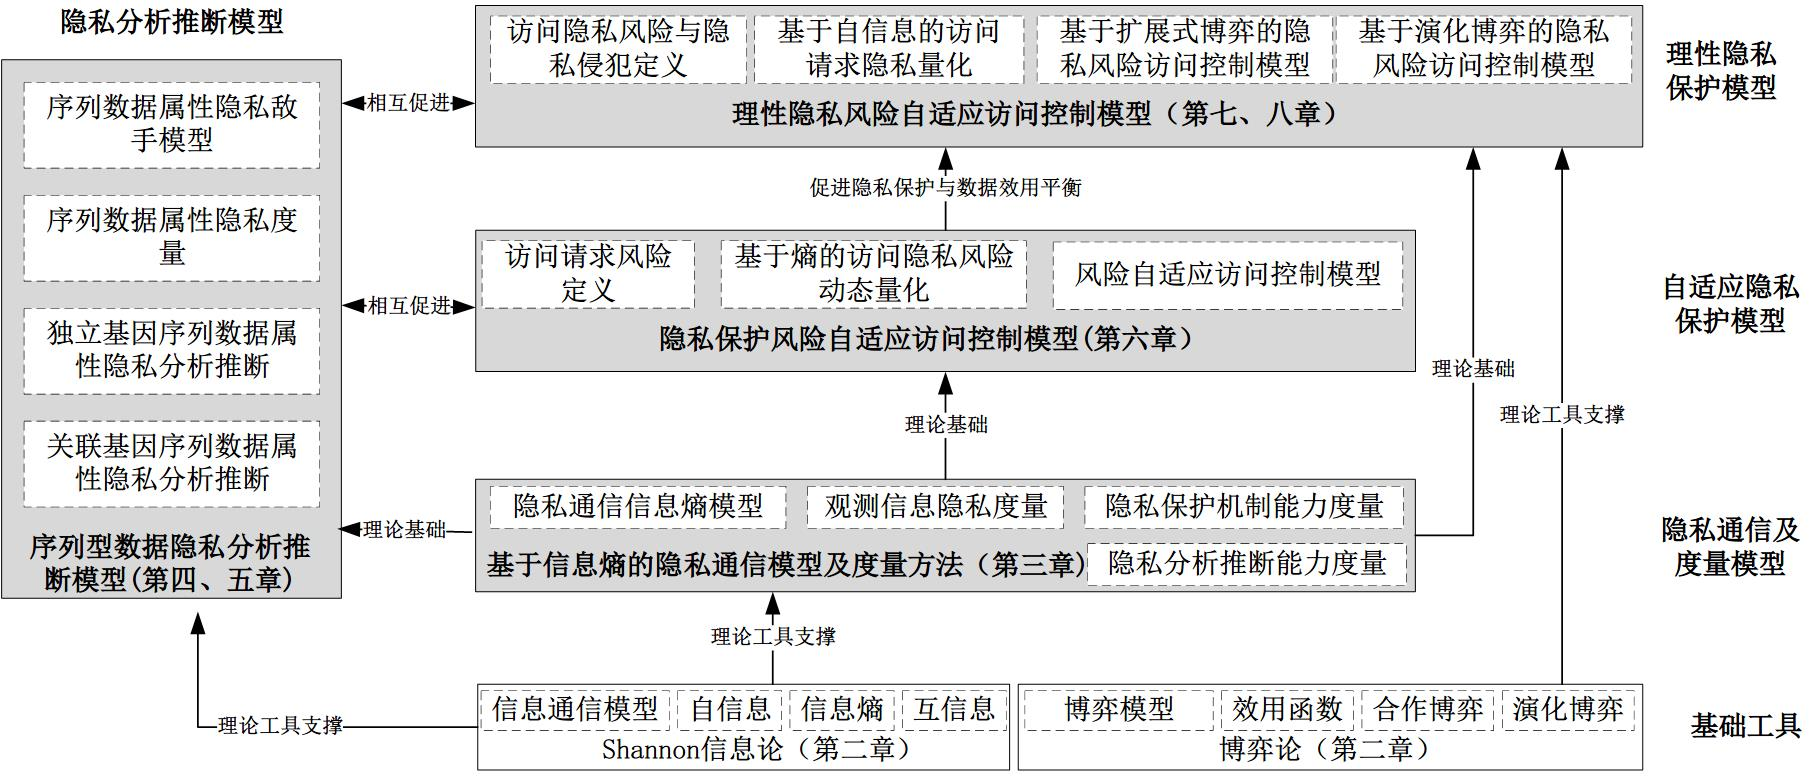
\includegraphics[width = 0.99\linewidth]{./figures/chapter1-research-framework.jpg}
	\caption{研究体系及论文结构安排}
	\label{fig:chapter1-research-framework}
\end{figure}

\textbf{1.	基于信息熵的隐私通信模型及度量方法}

利用信息论的相关工具,如熵、互信息等来对匿名隐私、成员关系隐私和属性隐私进行形式化定义和度量的研究较多,但是大部分是集中在位置匿名、轨迹匿名、数据集匿名、数据集成员属性、训练集关系隐私、社交网络匿名和属性等方面的研究。在隐私量化方面,缺乏对隐私定义、隐私分析、隐私保护等统一的量化方法。

本文基于Shannon信息论的通信模型框架提出了几种隐私保护信息通信模型,对不含敌手的隐私保护、含敌手的隐私保护、多隐私保护源的隐私保护等不同情境提出了相应的模型进行建模,以满足对隐私度量、隐私保护机制效果度量和敌手隐私分析强度度量等需求。在所提出的度量模型中,将信息拥有者假设为发送方,隐私谋取者假设为接收方,隐私的泄露渠道假设为通信信道;基于该假设,分别引入信息熵、平均互信息量、条件熵及条件互信息等来分别描述隐私保护系统信息源的隐私度量、隐私泄露度量、含背景知识的隐私度量及泄露度量,形成了以信息论为核心的隐私度量方法体系;以此为基础,进一步提出了隐私保护方法的强度和敌手攻击强度的量化,为隐私泄露的量化提供了一种支撑,对整个隐私保护过程中的保护机制、敌手能力都提供了量化方法。

在构建的隐私保护通信模型中,将含敌手的隐私保护机制构建了如图~\ref{fig:Communication-Model-for-Privacy-of-Single}所示的通信模型,并定义了信源熵、攻击条件熵、互信息量等来量化隐私。
\begin{figure}[htbp]
	\centering
	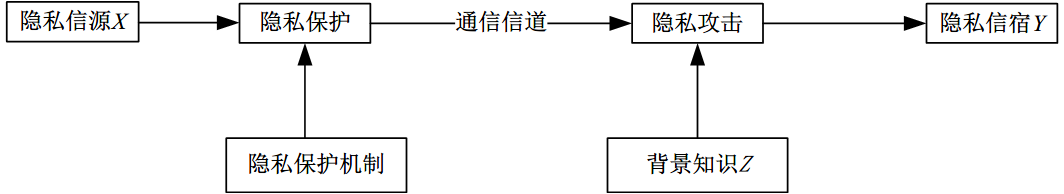
\includegraphics[width = 0.95\linewidth]{./figures/Communication-Model-for-Privacy-of-Single.png}
	\caption{单隐私信源且敌手具备知识背景的隐私保护通信模型}
	\label{fig:Communication-Model-for-Privacy-of-Single}
\end{figure}

针对该模型,隐私信源熵$H(X)$为
\begin{equation}
H(X)=-\sum_{i=1}^{n}p(x_{i})\log_{2}p(x_{i})
\end{equation}
~$H(X)$~用于刻画隐私信源的平均隐私信息量,也是隐私信源的隐私不确定程度,~$H(X)$~越大,隐私泄露就可能越小,从而它亦可以用于衡量隐私的保护程度,在没有外部条件影响时,该值是一个确定的值。

隐私攻击条件熵$H(X/YZ)$为
\begin{equation}
H(X/YZ)=\sum_{i=1}^{n}\sum_{j=1}^{m}\sum_{k=1}^{l}p(x_{i}y_{j}z_{k})\log_{2}p(x_{i}/y_{j}z_{k})
\end{equation}
~$H(X/YZ)$~反映了攻击者在获得隐私信宿消息~$Y$~和背景知识~$Z$~后,关于~$X$~仍存在的不确定度,它实际了可以作为在具有攻击分析的情况下隐私信息的不确定度,亦可以作为隐私保护强度的度量。

隐私攻击平均互信息$~I(X;Y/Z)$~为
\begin{equation}
I(X;Y/Z)=\sum_{i=1}^{n}\sum_{j=1}^{m}\sum_{k=1}^{l}p(x_{i}y_{j}z_{k})\log_{2}\frac{p(x_{i}z_{k}/y_{j})}{p(x_{i}/z_{k})p(y_{j}/z_{k})}
\end{equation}
该公式反映了得到~$Z$~的条件下,~$X$~和~$Y$~之间的平均互信息量,即接收方获得的隐私信息量,即可以刻画具有背景知识攻击下的隐私泄露程度。

在此基础上定义了隐私保护机制、隐私分析敌手攻击能力的量化方法,具体有:

对同一隐私信源~$X$~,其与隐私信宿~$Y$~进行通信过程中受到敌手应用隐私攻击进行攻击~$A_{r}$~,系统分别应用隐私保护机制~$P_{i}$~和~$P_{j}$~对隐私消息进行保护,若~$H_{P_{i},A_{r}}(X/YZ)<H_{P_{j},A_{r}}(X/YZ)~$(~$I_{P_{i},A_{r}}(X;Y/Z)<I_{P_{j},A_{r}}(X;Y/Z)$~),则称在抗~$A_{r}$~攻击下,隐私保护机制~$P_{j}$~比隐私保护机制~$P_{i}$\textbf{隐私保护有效性好},简记偏序关系~$P_{i}(A_{r})\prec P_{j}(A_{r})$~。若~$H_{P_{i},A_{r}}(X/YZ)=H_{P_{j},A_{r}}(X/YZ)~$(~$P_{P_{i},A_{r}}(X;Y/Z)=I_{P_{j},A_{r}}(X;Y/Z)$~),则称隐私保护机制~$P_{i}$~与隐私保护机制~$P_{j}$\textbf{隐私保护有效性}相等,简记等价关系~$P_{i}(A_{r})\cong P_{j}(A_{r})$~。


在含敌手攻击的隐私保护信息熵模型中,对同一隐私信源~$X$~,针对该信源的隐私消息有隐私攻击~$A_{r}$~,若在该隐私攻击下分别应用隐私保护机制~$P_{i}$~和~$P_{j}$~进行保护,隐私信源~$Y$~在该攻击下接收到的隐私信息量分别为~$I_{P_{i},A_{r}}(X;Y/Z)$~和~$I_{P_{j},A_{r}}(X;Y/Z)$~,则称两种隐私保护机制在隐私攻击~$A_{r}$~下的有效性距离为~$D_{i}(A_{r})=\left | I_{P_{i},A_{r}}(X;Y/Z)-I_{P_{j},A_{r}}(X;Y/Z) \right |~$~。

对同一隐私信源~$X$~,其与隐私信宿~$Y$~进行通信过程中应用隐私保护机制~$p_{i}$~进行隐私保护,并分别受到敌手应用隐私攻击~$A_{r}$~和~$A_{\alpha }$~进行攻击,若~${{H}_{{{P}_{i}},{{A}_{r}}}}(X/YZ)<{{H}_{{{P}_{i}},{{A}_{q}}}}(X/YZ)~$ (${{I}_{{{P}_{i}},{{A}_{r}}}}(X;Y/Z)>{{I}_{{{P}_{i}},{{A}_{q}}}}(X;Y/Z)$~),则称在隐私保护机制的保护下, 隐私攻击~$A_{r}$~比隐私攻击~$A_{\alpha }$~的隐私攻击有效性更强,简记偏序关系。若~$H_{P_{i},A_{r}}(X/YZ)<H_{P_{i},A_{q}}(X/YZ)~$(~$I_{P_{i},A_{r}}(X,Y/Z)<I_{P_{i},A_{q}}(X,Y/Z)$~),则称在隐私保护机制~$P_{i}$~的保护下, 隐私攻击~$A_{r}$~与隐私攻击~$A_{\alpha }$~的\textbf{隐私攻击有效性相同},简记等价关系~$A_{r}(P_{i})\cong A_{q}(P_{i})$~。

在含敌手攻击的隐私保护信息熵模型中,对同一隐私信源~$X$~的隐私消息应用隐私保护机制~$P_{i}$~进行保护,并有隐私攻击~$A_{r}$~和~$A_{\alpha}$~分别进行隐私攻击,隐私信源~$Y$~在不同攻击下接收到的隐私信息量分别为~$I_{P_{i},A_{r}}(X;Y/Z)$~和~$I_{P_{i},A_{q}}(X;Y/Z)$~,则称两种隐私攻击针对隐私保护机制~$P_{i}$~的有效性距离为
$D_{i}(P_{i})=\left | I_{P_{i},A_{r}}(X;Y)-I_{P_{i},A_{q}}(X;Y) \right |$。

在带敌手攻击的隐私保护通信模型中,隐私信宿~$X$~发送隐私消息,经过隐私保护和隐私攻击,被隐私信宿~$Y$~接收,若敌手已知背景知识空间~$Z$~,则~$I(X;Y)\leqslant I(X;YZ)$~。说明敌手在一定背景知识进行隐私攻击与分析, 敌手获得的隐私信息不少于其无背景知识情况下所能获得的隐私信息。同时也为隐私保护提供了一个方向,即尽可能使得敌手截取的隐私消息与其拥有背景知识关联程度尽可能小,从而最大限度的保护隐私信息。
	
\textbf{2.	独立序列型数据属性隐私推断模型}

近年来,由于数据种类繁多、数量庞大且应用需求多样化,越来越多的数据被以集中或分布式的形式共享、开放,造成了大量的隐私泄露,这些泄露又成为敌手进行隐私分析的背景知识,增加了数据共享的隐私泄露风险,对数据隐私泄露的潜在威胁量化,对数据隐私保护机制设计都提出了高的要求。特别是需要对隐私泄露的原理进行进一步研究,以帮助更好地度量隐私、理解隐私泄露机理,并设计更好的隐私保护方法。目前针对匿名方法的去匿名性分析研究较多,针对社交网络的用户偏好、个人信息等属性隐私的分析研究较多,但是对新型序列化数据的属性隐私,如时间序列的位置隐私、基因序列的基因座敏感值隐私较少,此类数据在很多共享应用场景(如疾病诊断、车联网导航)中需要非匿名化,需要对其敏感的属性隐私(特定基因座的基因型,特定行车位置)进行保护。

本文针对基因序列数据的属性隐私提出了一种基于概率推断的隐私分析模型。该模型通过对单条敏感数据记录属性值存在的相互关联关系进行分析,构建目标属性值推断的敌手模型。在提出的敌手模型基础上,分别提出了两种不同的基因序列属性隐私分析方法。第一种主要基于Monte Carlo-Markov抽样和隐Markov推断算法,建立了目标基因序列的“抽样解析”——“单倍体属性值概率推断”——“二倍体合成”三个步骤的属性隐私推断模型;第二种方法应用卷积神经网络构建概率推断算法,改进了单倍体属性值推断过程,实现了大规模序列型数据的属性推断目标。所提出的方法针对不存在亲属关系的群体基因序列数据共享场景,在本文提出的隐私度量模型基础上,定义了序列型数据属性隐私和量化方法,并应用于分析属性隐私泄露情况,通过量化隐私泄露量和敌手获取隐私量等信息,提高对序列型数据属性隐私的认识和理解。实验表明,本文提出的方法比现有基因序列属性隐私分析模型和算法更优,敌手对属性隐私的错误率、不确定度降低,敌手获得隐私信息量都比已有的工作更优。

在所提出的序列型数据属性隐私推断模型中,提出了如图~\ref{fig:adversary-model} 所示的敌手模型。由于隐私保护的需求,被攻击者希望隐藏某些可能与遗传病或私人特征有关的敏感SNP。因此,被攻击对象共享其原始SNP序列的变体~$\hat{X}=(\hat{x}_1,\hat{x}_2, ... , \hat{x}_n)$~, 其中~$\hat{x}_i =\{0,1,2\}$~,并隐藏其中某些SNP。假设隐藏的SNP用~$X_h$~表示,可观测的SNP用~$X_O~$~表示,公开的SNP用~$X=(x_1, x_2, ..., x_n)=X_H \cup X_O~$~,其中~$X_i =\{-1,0,1,2\}$~,值~$X_i=-1$~表示~$X_i\in X_h$~是隐藏的SNP。假设已观测被攻击者公开SNP$~X$~序列数据的敌手想要重构原始SNP序列~$\hat{X}$~。为此,敌手可以通过推断攻击获取被攻击者的基因组隐私(例如获得其APOE基因状态)。要进行这样的推断攻击,敌手将收集一些公开可用的基因组信息,例如被攻击者所属族群的次要等位基因频率(Minor Allele Frequency,MAF)、LD值、遗传重组率和单倍体基因型参照。

\begin{figure}[htbp]
	\centering
	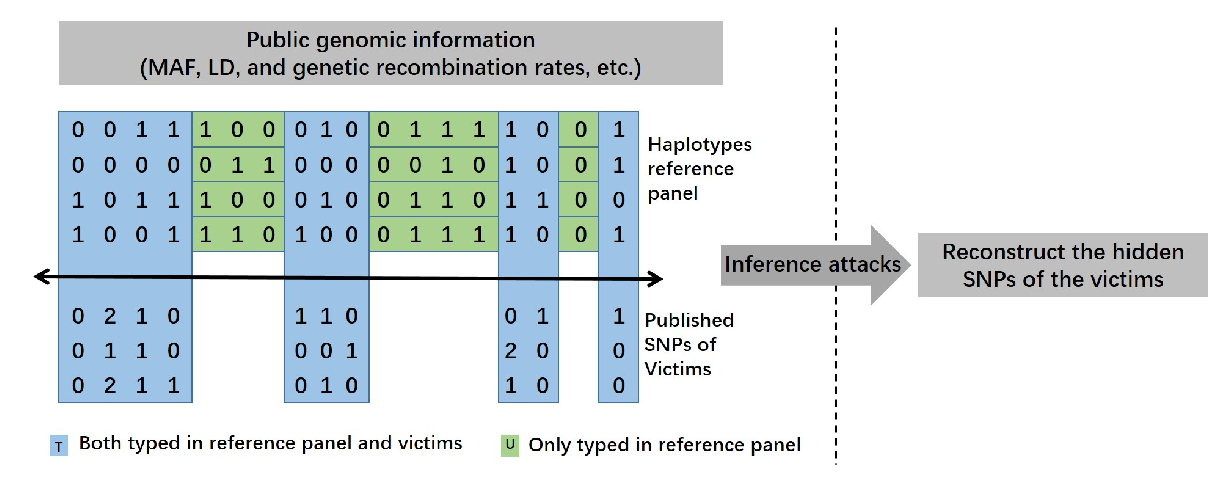
\includegraphics[width = 0.95\linewidth]{./figures/Fig2-adversary-model}
	\caption{基因序列数据属性隐私分析推断敌手模型概览}
	\label{fig:adversary-model}
\end{figure}

在此敌手模型下,基因序列数据属性隐私推断攻击可以看作是给定已发布的SNP和公开基因组信息,计算每个隐藏SNP的条件边缘概率分布的过程,即
\begin{equation}
Prob(X=\{0,1,2\})=Prob(X|(X_O,{INFOR}_{Pub})).
\end{equation}

基于iHMM的隐私序列数据隐私分析攻击可以分三个步骤进行,即

\begin{enumerate}
	\item[(1)] 敌手根据观测到的被攻击者的基因型数据,随机产生~$H_V^T$~的单倍型。然后,敌手通过多轮Markov链Monte Carlo迭代更新~$H_V^T$~中的单倍型。在每次迭代中,敌手通过从~$p(H_{V,i}^T|G_{V,i}^T,H_{V,-i}^T,H_R^T,\rho)$~中抽样来更新第~$i$~个被攻击者的阶段性单倍型对~$H_{V,i}^T$~。
	\item[(2)] 敌手通过基因重组模型利用HMM模型推断~$H_V^u$~中的单倍型。在每次迭代中,敌手根据条件概率分布~$p(H_{V,i}^U|H_{V,i}^T, H_R^{T \cup U},\rho)$~推断第~$i$~个被攻击者对应~$U$~中的SNP序列的隐藏单倍型对~$H_{V,i}^u$~。 
	\item[(3)] 敌手把对每个被攻击者推断出来的单倍型对组合起来,得到被攻击者隐藏的SNP序列的推断基因型。
\end{enumerate}

基于RCNN的序列型数据属性隐私推断攻击,可将上述过程的步骤(2),改变为如图\ref{fig:rcnn_infer}所示神经网络训练与推测过程。

\begin{figure}[htbp]
	\centering
	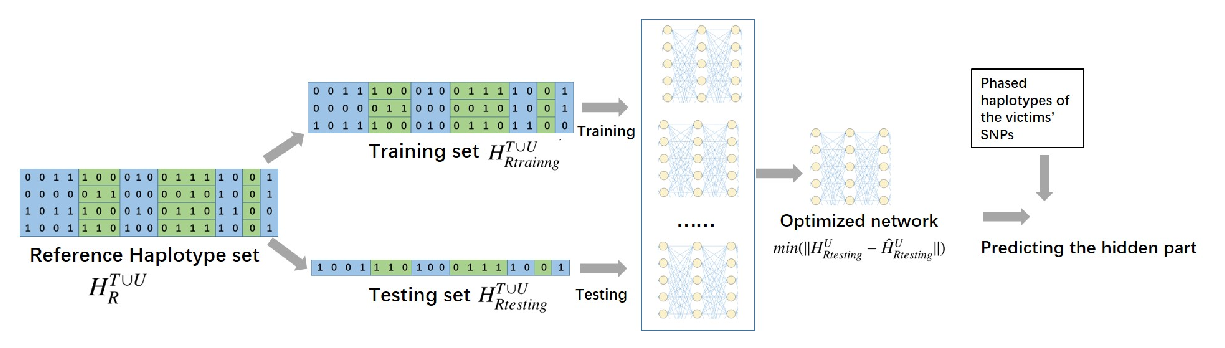
\includegraphics[width=0.95\linewidth]{./figures/Fig3-RCNN-inference-attack.eps}\\
	\caption{基于RCNN的隐私分析模型}
	\label{fig:rcnn_infer}
\end{figure}

通过实验结果分析,提出的两种隐私分析攻击方法,敌手能够准确、低不确定性和高隐私损失地推断出个体的私有隐藏SNP隐私信息。所提出的攻击扩展并显著改进了现有的工作。通过基于公开的基因组数据对个体基因组隐私进行量化,该工作可以帮助人们更好地理解当前基因组隐私面临的风险,促进隐私领域更加小心地应用基因组数据,促进研究人员设计更好的隐私保护模型(如后文研究的基于风险访问控制模型)以适应性地保护基因序列数据隐私。

\textbf{3.	关联序列型数据属性隐私推断模型}

随着不同机构和个人更加容易获取基因组数据,且这些敏感数据被广泛地应用于医疗、保险、寻亲及社交等场景,对数据安全和隐私的担忧也在不断加剧。为了证实在序列型数据属性隐私方面,存在个人共享基因数据也会大量泄漏他人属性隐私的问题,为了进一步分析家族成员基因序列数据共享会造成他人基因序列属性隐私泄露的机理,需要对相互关联的基因序列型数据进行隐私分析。

本文利用因子图和置信传播算法针对亲属间的基因序列属性隐私建立分析推断敌手模型和分析算法。该模型考虑了单核苷酸多态性间高阶相关性,利用公开DNA参照数据集和全基因组关联研究(GWAS)目录数据,提高了推断攻击模型的属性隐私分析强度。该模型的敌手隐私分析强度通过本文所提出的隐私度量框架,对基因序列属性隐私进行了定义,并将隐私损失量作为评价指标进行了隐私分析强度量化。实验结果表明,所提出的攻击更适合于高密度基因组数据隐私推断,且具有较少的错误率、不确定性和更多隐私损失,显著提高了属性隐私的隐私分析推断能力。

所提出的敌手模型中敌手的目的是通过使用 (i) 观测到的一个或多个家庭成员的基因组数据 (即 SNP序列),  (ii) 观测到的一个或多个家庭成员的基因组相关特征和疾病, (iii) 家族的谱系结构, (iv) 遗传规律,特别是孟德尔遗传定律, (v) 核苷酸的次要等位基因频率 (MAF) 或等位基因频率, (vi) SNP之间的族群LD值, (vii) 族群的SNP, (viii) GWAS目录,以及 (ix) 遗传疾病的发病率等信息,推断被攻击者的SNP,身体特征和疾病。属性隐私分析框架如图\ref{fig:attack-framework} 所示。
\begin{figure}[htbp]
	\centering
	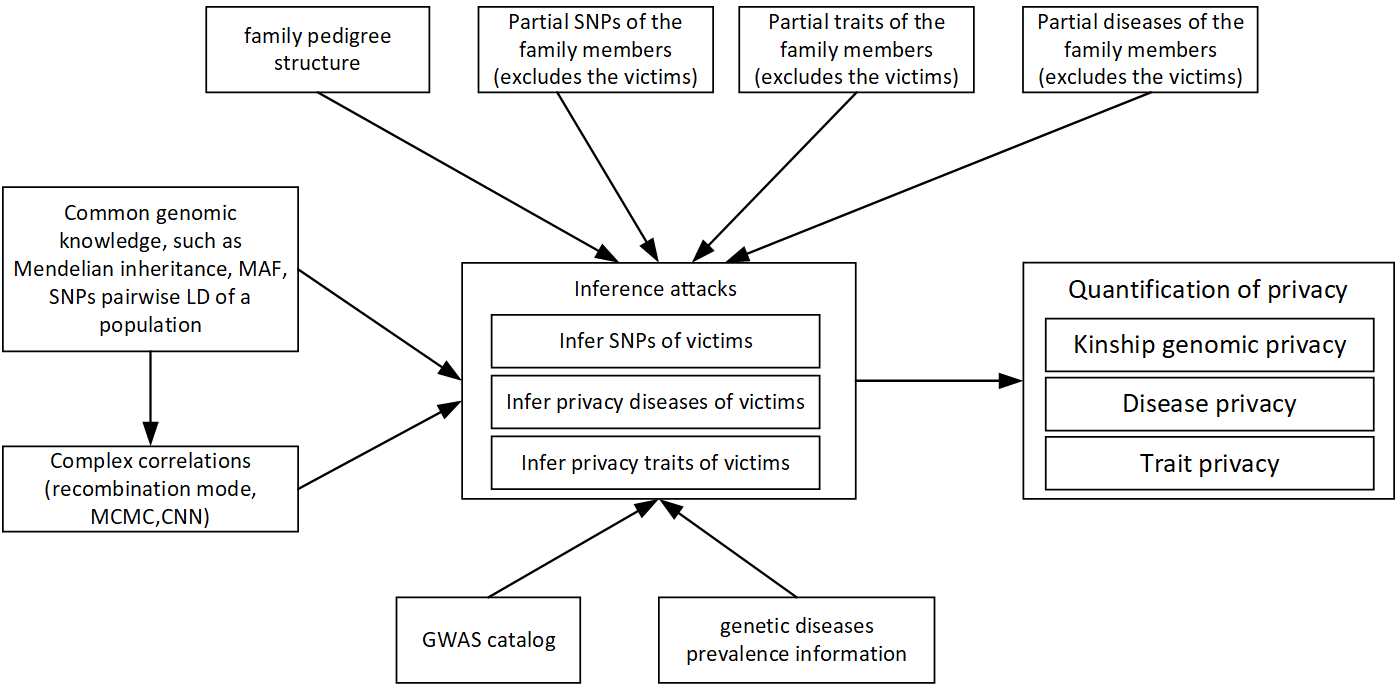
\includegraphics[width=0.95\linewidth]{./figures/attack-framework.png}
	\centering
	\caption{亲属基因组属性隐私分析推断框架}\label{fig:attack-framework}
\end{figure}

若将家庭成员~$i$~的SNP ~$j$~的边缘分布表示为~$p(x_{ij})$~,则~$\mathbf{X}_u$~的每个变量的边缘概率分布可以得到为
\begin{equation}
p(x_{ij})= \sum_{\mathbf{X}_U/\{x_{ij}\}} p(\mathbf{X}_U | \mathbf{X}_K, \mathbf{T}_K, \mathbf{D}_K, T,  \mathcal{F}_T(x_i^F,x_i^M,x_i^C), \mathbf{P}, \mathbb{T}, \mathbb{D}, \mathbb{P}, \mathbf{F})
\end{equation}
我们为概率推断计算建立一个因子图以提高实际隐私分析算法计算效率。该图具有两种类型的节点(变量节点和因子节点)和连接节点的边。在此因子图中设置了每个SNP ~$x_{i,j}$~的变量节点(~$x_{i,j}\in \mathbf{X}$~,~$i$~表示家庭成员ID,~$j$~表示家庭成员~$i$~的SNP ID)。本模型使用四种类型的因子节点:(i)\emph{家族因子节点},代表家族关系(关于孩子和父母)和遗传,(ii)\emph{重组模型相关因子节点},代表SNP之间的重组模型相关性,它比其他类型的高阶相关性包含更多的信息,(iii)\emph{特征因子节点}代表SNP与个体特征之间的关系,以及(iv)\emph{疾病因子节点},代表SNP与个体基因组疾病之间的关系。变量和因子节点之间的联系描述如下。

\begin{itemize}
	\item 每个变量节点~$X_{i,j}$~具有其家族因子节点~$f_{i,j}$~,且二者相互连接。 若~$k$~是家庭中~$i$~的父母,则~$x_{k,j}$~(~$k \neq i$~)也连接到~$x_{i,j}$~。 若所观测到的家庭中~$i$~的父亲或母亲都没有,则因子节点~$f_{i,j}$~的度为1; 若只有~$i$~的父亲或母亲,则因子节点~$f_{i,j}$~的度为2; 若被观测家庭中有双亲~$i$~,则该度为3。 如图3中的示例所示,孩子的家庭因子节点的度数为3,因为他的父母都在这里,而父母的家庭因子节点的度数均为1,因为父亲或母亲的父母都未出现在被观测家庭中。
	\item 集合~$\mathbf{C}$~中的变量节点连接到重组模型相关因子节点~$rf_{i,\mathbf{C}}$~。 由于我们使用重组模型来训练SNP之间的相关性,因此所有SNP都可以视为与重组能力相关。设~$\mathbf{C}$~等于~$\mathbf{x}$~,其中包括一个人的所有SNP。 另一方面,Markov假设可以提高效率。 我们在实际计算步骤中使用基于Markov的计算方法。
	\item 若~$\mathbf{T}_{i,\alpha}$~中的SNP与特征~$T_{\alpha}$~( ~$T_{\alpha} \in \mathbf{t}$~)相关联,则集合~$\mathbf{T}_{i,\alpha}$~中的家族成员~$i$~的可变节点连接到特征因子节点~$tf_{i,\alpha}$~。 ~$\mathbf{T}_{i,\alpha}$~和 ~$\mathbf{T}_{j,\alpha}$~ (~$i \neq j$~)的SNP具有相同的基因座集合。 这意味着对于不同个体的特定特征,相关SNP的位点是相同的。 ~$\mathbf{T}_{i,\alpha}$~中的SNP数量可能大于1。换句话说,一个给定的性状与一个以上的SNP相关;另外,一个SNP也可能与一个以上的性状相关。 有时已经观测到家族成员的某些特征,有时没有。
	\item 若~$\mathbf{D}_{i,\beta}$~中的SNP与遗传疾病~$D_{\beta}$~(~$D_{\beta} \in \mathbf{d}$~)相关,则~$\mathbf{D}_{i,\beta}$~组中家族成员~$i$~的变量节点连接到性状因子节点~$df_{i,\beta}$~。 类似地,可能有不止一种SNP与给定的遗传疾病相关; 一个SNP也可能与一种以上疾病有关。有时已经从家族成员身上观测到了某些疾病,有时则没有。值得注意的是,对于特定疾病,即使相关SNP的位点对于不同的个体而言都是相同的,该疾病的当前结果也有所不同,因为该疾病也可能受到其他因素的影响。
	
\end{itemize}


\textbf{4.	隐私保护风险自适应访问控制模型}

在以数据为中心的开放系统中,数据往往通过云服务或其他集中式的方式按需提供数据共享、开放、应用服务,这些需求多样复杂产生了复杂的隐私泄露风险和威胁,需要动态化、细粒度、适应性的方案对数据提供访问控制模式的隐私保护。但目前基于传统的强制访问控制、基于角色访问控制以及新型的基于属性访问控制,都不能很好的解决该问题。

本文针对云环境中共享、应用涉及隐私或敏感信息数据的场景研究面向隐私保护的访问控制模型。在XACML上扩展提出了一种基于风险的自适应访问控制模型,以动态化地在访问控制过程中保护数据隐私,约束隐私侵犯行为,激励诚实访问行为。首先,根据风险访问控制场景的隐私保护需求提出了面向隐私保护的风险访问控制敌手模型;其次,该模型在标准的XACML框架进行了扩展,新增了策略风险评估、会话控制和风险消减服务三个组件,增强了策略执行、策略访问和策略信息组件。在新增的组件中,以Shannon信息熵作为工具,在提出的隐私度量模型基础上,提出了基于风险的隐私定义和量化方法,对用户的访问控制请求风险和用户自身的风险类型结合,提出了访问请求类型判别方法;通过风险隐私量化及基于信用卡模型的激励机制,实现访问行为风险阈值的动态调整,考虑了用户短期访问行为和长期访问行为的影响。对比和分析表明,所提出的模型和方法较现有的工作更加动态化,且实现了隐私保护,易用性更好。

在所提出的隐私保护访问控制模型中,其主要组件和流程如图\ref{fig:Process_flow}所示。

\begin{figure}[htbp]
	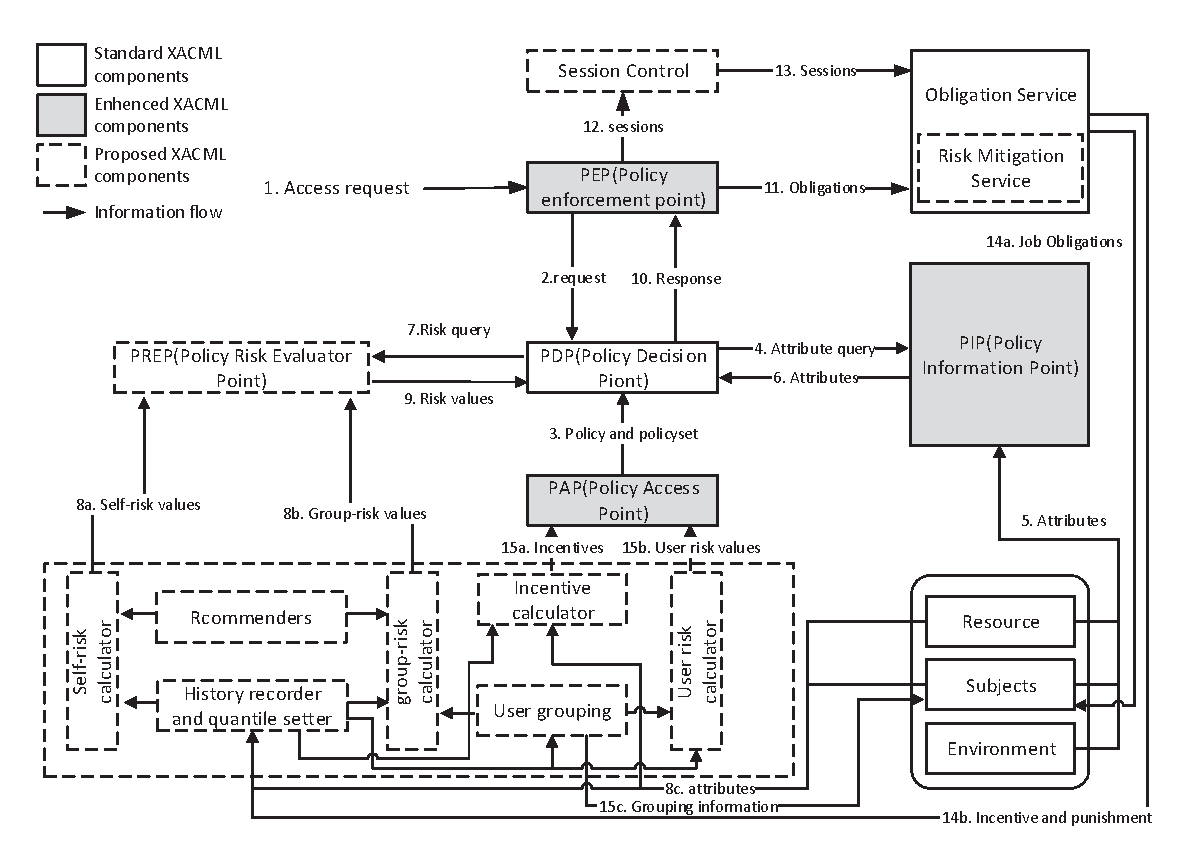
\includegraphics[width=\linewidth]{./figures/Process_flow.eps}
	\caption{基于XACML的风险自适应访问控制框架流程}
	\label{fig:Process_flow}
\end{figure}

其中,用户$u$的第$n$次访问请求$q_n$的自访问风险值可表示为
\begin{equation}
\label{eq:self risk 3}
sr(u,q_n)=
\left\{
\begin{array}{ll}
I(q_i)=-logp_i, & \hbox{是否有足够的历史数据;} \\
Avg(I(u,q)), & \hbox{若历史还不够;} \\
1, & \hbox{若没有可用的历史数据。}
\end{array}
\right.
\end{equation}

用户$u$的第$m$次访问请求$q_n$的组访问风险值~$gr(g,q_m)$~可计算为
\begin{equation}
\label{eq:group risk}
gr(g,q_m)=
\left\{
\begin{array}{ll}
I(q_i)=-logp_i, & \hbox{若有足够的历史数据 ;} \\
Avg(I(g,q)), & \hbox{若历史数据不够;} \\
1, & \hbox{若没有可用的历史数据。}
\end{array}
\right.
\end{equation}
数据服务提供者或系统可以根据请求的风险级别做出访问控制决策,即
\begin{equation}
\label{eq:decision}
decision=
\left\{
\begin{array}{ll}
p, & \hbox{若~$q$~为自正常访问请求,且为群组正常访问请求;} \\
p(rm), & \hbox{若~$q$~为自风险访问请求,但为群组正常访问请求;} \\
d, & \hbox{若~$q$~为自风险访问请求,且为群组风险访问请求;} \\
d(p), & \hbox{若~$q$~为自正常访问请求,但为群组风险访问请求。} \\
\end{array}
\right.
\end{equation}

\textbf{5.	基于扩展式博弈的理性隐私风险访问控制模型}

基于风险访问控制模型可很好的解决以数据为中心的开放系统中自适应数据隐私保护。但强制访问控制、基于角色访问控制、基于属性访问控制和已有的基于风险访问控制等模型,在平衡隐私保护需求与数据效用需求冲突方面,仍存在问题,特别是过度授权导致隐私泄露或授权不足导致数据可用性不足的问题需要进一步解决。此外,还需要对基于风险访问模型中对隐私保护的能力和方法进一步提升。

针对上述需求和问题,本文在所提出的风险自适应访问控制模型的基础上,进一步运用Shannon自信息和博弈论,提出了基于风险适应性的理性访问控制模型以实现数据共享场景中的保护隐私和数据应用需求间的平衡。在定义了隐私风险和隐私侵犯访问的概念之后,提出了基于博弈论的风险访问控制模型框架和工作流程,其中模型框架如图\ref{fig:game-rbac-framework}所示。此外,还进一步利用Shannon信息的定义提出了量化访问请求隐私风险和用户隐私风险值的计算公式,强化了访问控制请求对数据隐私的刻画;以提出的理性风险访问控制模型、访问请求隐私 风险和用户隐私风险为基础,提出了多轮二人博弈来刻画面向隐私保护的风险访问控制中访问者与数据服务提供者的“隐私保护-数据服务”冲突与合作关系,进一步提出并分析了博弈效用函数及其二人博弈过程。分析表明,在基于隐私风险访问控制的每一轮博弈中都存在子博弈精炼纳什均衡,可以通过限制侵犯隐私的访问请求来保护隐私,实现隐私保护与数据访问效用间的平衡。分析和对比表明,该方法比已有的工作更有优势,需要更少的辅助信息,提供更多的风险适应性和隐私保护强度。

\begin{figure}[htb]
	\centering
	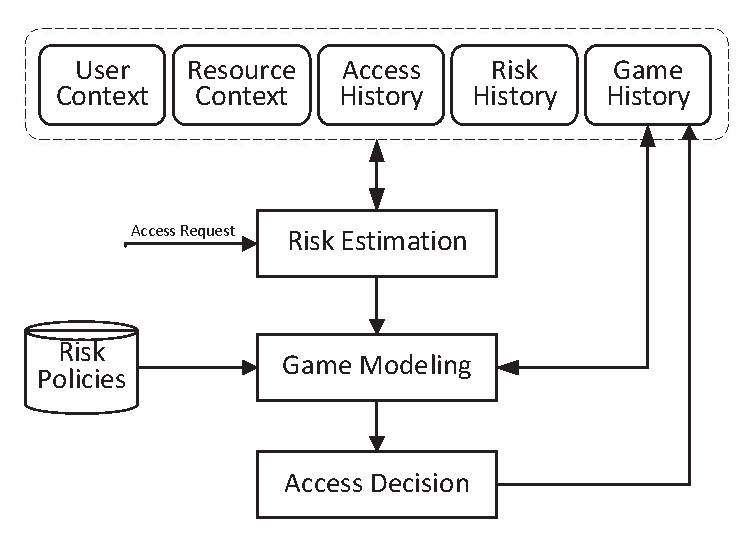
\includegraphics[width=.65\textwidth]{./figures/game-rbac-framework.eps}
	\caption{基于博弈论风险适应性访问控制框架 (RaBAC)}\label{fig:game-rbac-framework}
\end{figure}
该模型中,通过使用~$r_{q_U}$~的自信息和~$r^g_i$~的平均信息之间的距离来量化\emph{访问请求隐私风险} ~$r_{q_U}$~,如下
\begin{equation}\label{eq:privacy_risk_qu}
r_{q_U} = \dfrac{|Infor(R_{q_U})-\dfrac{\sum ^{n}_{i=1} Infor(R^g_i)}{n}|}{\dfrac{\sum ^{n}_{i=1} Infor(R^g_i)}{n}}, 
\end{equation}
将用户的风险$r_U^{i}$计算为
\begin{equation}\label{eq:userrisk}
r_U^{i}=\left\{ 
\begin{array}{cl}
r_U^{i-1}(1-\dfrac{\alpha}{r_{max}}), & \text{若 } q_U \text{是正常访问请求;}\\
r_U^{i-1}(1+\dfrac{\beta}{r_{max}})), & \text{反之。}
\end{array}
\right.
\end{equation}

将基于风险适应性的访问控制建模为一种隐私保护的博弈模型,其中涉及参与者、参与者策略和参与者效用函数。在这个博弈中,有两个参与者,服务提供者~$S$~和用户~$U$~。服务提供商拥有隐私敏感的资源(即访问客体),并希望授权正常访问请求并拒绝侵犯隐私的访问请求;用户是访问主体,其因为经济或其他利益而希望尽可能多地访问这些访问客体。用户~$U$~有两种策略,执行正常访问~$N$~和执行违反隐私的访问~$V$~;服务提供商~$S$~有两种策略,分别授权正常请求~$G$~和拒绝正常请求~$D~$~。
该博弈模型是一个多次博弈过程,可以分别考虑每次博弈的策略选择关系,并将每个子博弈视为一个独立博弈。假设此博弈中有~$T$~次子博弈,且~$\sigma_1^*, \sigma_2^*, \cdots, \sigma_T^*$~是独立阶段博弈的Nash均衡策略的有序序列,然后该序列存在子博弈完美均衡,且均衡路径由~$\sigma_1^*, \sigma_2^*, \cdots, \sigma_T^*$~生成。在每个阶段的博弈中都会求得最佳策略选择解。服务提供商和用户都可以获得最大的收益,且单次子博弈都可以达到Nash均衡。因此,用户将执行正常访问,而服务提供商将准许用户的正常访问请求。 因此,服务提供商通过限制隐私侵害访问来保护信息资源中涉及的隐私信息。

\textbf{6.	基于演化博弈的理性隐私风险访问控制模型}

社交网络、医疗信息系统等以数据为中心的大规模用户(访问者)开放信息系统,亟需能够保护隐私的细粒度自适应访问控制模型,且需实现数据隐私保护需求和数据效用需求的平衡。现有基于理性的访问控制模型难以满足适应性保护隐私的需求,且博弈参与者的完全理性假设太强,不符合实际场景。基于风险访问控制能够实现细粒度的访问控制隐私保护目标,但如何进一步放松参与者完全理性的假设,并实现隐私保护与数据效用关系的动态平衡,仍需要进一步研究。

\begin{figure}[htbp]
	\centering
	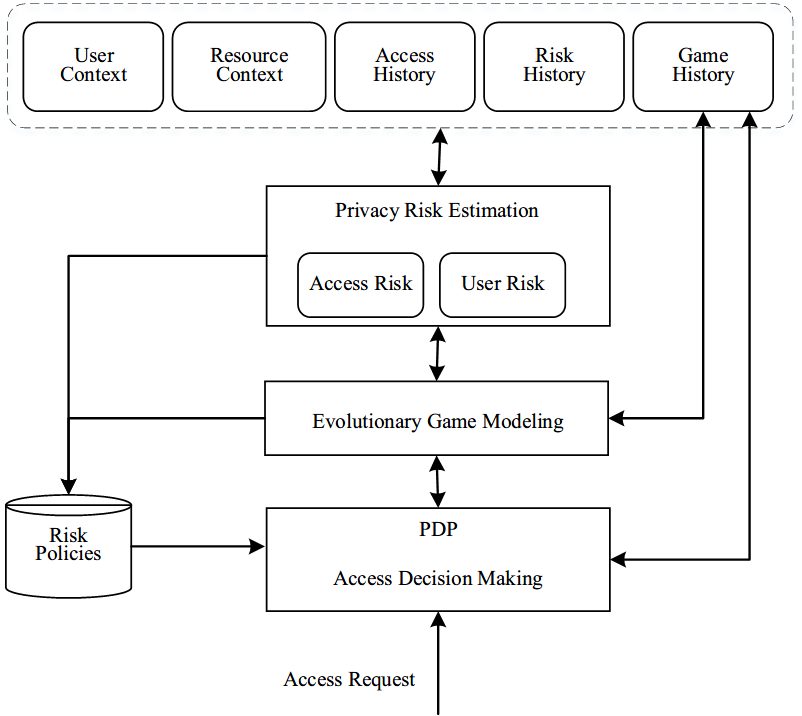
\includegraphics[width = 0.6\linewidth]{./figures/Evolutionary-game-Rabac.png}
	\caption{基于演化博弈的隐私风险访问控制模型}
	\label{fig:Evolutionary-game-Rabac}
\end{figure}

针对这些问题和需求,在提出的风险自适应访问控制模型和完全理性隐私风险访问控制模型的基础上,进一步提出一种面向隐私保护的有限理性风险自适应访问控制模型,如图\ref{fig:Evolutionary-game-Rabac}所示。新提出的模型包含了新的隐私风险量化模块和演化博隐私弈决策模块。该模型首先基于信息量对访问请求的数据集隐私信息量进行量化,构造了访问请求隐私风险函数和用户隐私风险函数;其次,基于演化博弈在有限理性假设下构建多参与者的访问控制演化博弈模型,利用复制动态方程分析了访问控制参与者的动态策略选择和演化稳定状态形成机理,提出了隐私风险访问控制博弈演化稳定策略的选取方法。仿真实验和对比表明,所提出的访问控制模型能够有效动态自适应地保护敏感信息资源系统中的隐私信息,具有更好的隐私风险适应性,有限理性参与者的动态演化访问策略选取更加符合实际场景。

在该模型中,用户~$U$~的当前访问请求~$q_{0}^{U}$~隐私风险为

\begin{equation}
r(q_{0}^{U})=\begin{cases}
1, & \text{ 若 } R_{0}^{U}/{{R}^{g}}\ne \varnothing \\ 
\alpha \frac{-|R_{0}^{U}/{R}^{U}|max_{x\in R_{0}^{U}/{R}^{U}}logp(x)}{-\sum_{x\in{R^U}}logp(x)}+ \beta \frac{-\sum_{x\in R_0^U \cap  R^U}logp(x)}{-\sum_{x\in  R^U}logp(x)}& \text{若 } R_{0}^{U}/{{R}^{g}}=\varnothing 
\end{cases}
\end{equation}

当前访问请求~$q_{0}^{U}$~发出之后,系统根据其隐私风险值~$r_{n}^{U}$~和访问请求~$q_{0}^{U}$~的隐私风险值~$r(q_{0}^{U})$~计算用户~$U$~的更新隐私风险值

\begin{equation}\label{eq:users-risk}
r_{n+1}^{U}=\begin{cases}
r_{n}^{U}+r(q_0^U), & \text{ 若 } q_0^U \text{是一个隐私侵犯访问请求}; \\ 
r_{n}^{U}-r(q_0^U),& \text{反之。}
\end{cases}
\end{equation}

在此基础上,构建了基于风险访问控制的演化博弈模型,即,风险自适应访问控制演化博弈模型,可表示为4元组~$raBACEGM=(P,A,\Pr ,u)$~。
\begin{enumerate}
	\item ~$p=\{U,S\}$~是演化博弈的参与者空间,其中~$U$~是用户,~$s$~是信息资源系统。
	\item ~$a=\{{{A}_{U}},{{A}_{S}}\}$~是博弈策略空间,其中~${{A}_{U}}=~$~ ~$\{Normal,Malicious\}$~是用户的可选策略集合,包含正常访问和恶意访问两种,~${{A}_{S}}=\{Grant,Deny\}$~是信息资源系统的可选策略集合,包含授权和拒绝两种。
	\item ~$\Pr =\{p,q\}$~是博弈信念集合,其中~$p=\{{{p}_{Normal}},{{p}_{Malicious}}\}$~表示用户分别采取正常访问和恶意访问的概率,且~${{p}_{Normal}}\text{+}{{p}_{Malicious}}=1$~;~$q=\{{{q}_{Grant}},~$~ ~${{q}_{Deny}}\}$~表示信息资源系统分别采取授权和拒绝的概率,且~${{q}_{Grant}}+{{q}_{Deny}}=1$~。
	\item ~$u=\{{{u}_{U}},{{u}_{S}}\}$~是博弈参与者的收益函数集合,其中~${{u}_{U}}\text{= }\!\!\{\!\!\text{ }u_{U}^{N,G}\text{,}u_{U}^{N,D},u_{U}^{M,G},u_{U}^{M,D}\text{ }\!\!\}\!\!\text{ }$~是用户的收益函数,~${{u}_{S}}\text{= }\!\!\{\!\!\text{ }u_{S}^{N,G}\text{,}u_{S}^{N,D},u_{S}^{M,G},u_{S}^{M,D}\text{ }\!\!\}\!\!\text{ }$~是信息资源系统的收益函数,二者的值由参与者的访问策略选择所决定。
\end{enumerate}

给定不同的策略选取初始状态,经过演化,所提出的风险自适应访问控制模型在演化博弈过程中会达到某个稳定状态。通过对比,本演化博弈模型的模拟演化结果与理论分析保持一致,说明该演化博弈模型与现实系统中的规律相符。所提出的风险自适应访问控制演化博弈模型具有有效性,可将其应用于面向隐私保护的风险自适应访问控制系统中,为访问控制系统的参与者进行隐私保护访问策略选取提供依据。

\keywords{隐私度量,隐私推断分析,理性隐私保护,信息论,博弈论}


\newpage
  \begin{center}
	\heiti\zihao{-2}
	{Rational Privacy Preserving Model and Its Application}\\
	\heiti\zihao{4}
	{Summary}
\end{center}


With the rapid development of Internet, mobile Internet and Internet of things, as well as the continuous promotion of 5G technology and commercial promotion, massive data such as social network, location service, medical and health, biological gene and industrial control have been collected, transmitted, stored, transferred, analyzed and applied actively or passively.The generation and application of massive data have promoted the explosive growth of emerging industries and technologies such as cloud computing, big data and edge computing, and generated different applications such as smart medical treatment, smart transportation, smart government and smart city, greatly enriching people's material and spiritual life.Similarly, new changes such as quantitative growth of data, ubiquitous network across domains, cloud-based computing and diverse and complicated applications have brought huge challenges to security and privacy. A large number of viruses, vulnerabilities, attacks and data correlation analysis have led to serious privacy leakage, causing great concern among people.In recent years, various major privacy leakage events have fully demonstrated that privacy leakage has become an important threat in cyberspace. In this context, a deep understanding of privacy and privacy protection has become particularly important.

More than 90\% of data are collected and stored by governments, social organizations and enterprises providing public services, in order to give full play to the value of data, it is often necessary to share, open, exchange and analyze data containing a large amount of private information. At the same time, many information services are also based on the exchange of personal privacy information and service quality, such as website registration service, public WIFI access, cloud storage, smartphone navigation, information search and advertising push, online credit card payment, RFID application, etc. These scenarios due to regulatory requirements and individual desire, need to protect privacy information service providers at the same time, the data using the party or malicious third party want to get more privacy sensitive information, to provide better service, to obtain more data value, better data, two targets at the same time exists and conflict each other, need a balanced solution.

In 2006,  $k$-anonymous model was put forward after gradually become a systematic study of personal information, research and development, and based on the cryptography scheme based on cryptography two categories, these solutions are large used in data-centric open, complex and cross-domain scenario, as a cloud storage, social networks, location-based services, Internet of things, edge calculation, data mining, machine learning, health, etc.In many application scenarios, there is a natural contradiction between privacy protection target and data utilization target. How to balance the relationship between the two is one of the core problems.In these two types of privacy studies, the cryptographic-based schemes usually use the provable security theory to define the privacy protection objectives in the cryptographic sense, and design corresponding cryptographic schemes, such as state encryption, searchable encryption and attribute cryptography schemes, to achieve the privacy protection objectives.The scheme based on non-cryptography mainly defines the anonymous design algorithm to achieve the effect of anonymity to achieve the anonymous user identity privacy protection; By defining the indiscernibility of query results of adjacent data sets, a noise method is designed to achieve this indiscernibility to realize privacy protection of attribute values. By defining data dynamic privacy, fine-grained access control for adaptive risk is designed to protect private data from unauthorized users. Among them, the scheme has the strict theoretical method based on cryptography, can meet the expected targets of privacy protection, but the privacy is defined as security cryptography sense definition, privacy protection scheme design also rely on public key cryptography, the calculation for highly complex lead to inefficient, and difficult to compromise measures was adopted to realize data privacy protection and utility of balance; The scheme based on non-cryptography defines the privacy in the sense of anonymity and indiscernibility through probability or information theory, and designs the way of generalizing anonymity or adding noise to realize the privacy protection of anonymity or attribute value, which is efficient and conducive to balancing the effect of privacy protection and data utility. Currently, open a data-centric application scenario diversification, especially open sharing data applications, the mass under the premise of personal privacy need to ensure that data is available to get practical privacy protection, the research based on the cryptography scheme can achieve this goal, balance data privacy protection and utility, has the important practical significance.

There are three main scientific problems with privacy research. \textbf{First, privacy definition and measurement.} how to properly formalize the definition and quantification of privacy. In particular, privacy quantification includes not only the quantification of privacy in a particular data set, but also the quantification of privacy intensity in a certain privacy protection model, including the potential amount of personal privacy leakage and the assessment of privacy leakage after a privacy analysis attack model. \textbf{Second, privacy analysis and inference.} in a certain scenario, privacy analysis and inference are conducted for the data set of protected privacy information, and how to obtain more privacy information to the maximum extent. \textbf{Third, privacy protection}. How to effectively protect the privacy data set in a certain scenario and how to balance the effect of privacy protection and data utility while protecting privacy? In-depth study science problems and scientific problem two help understanding and awareness of privacy to researches in the mechanism of privacy, and to provide scientific theoretical basis for designing better privacy protection scheme and evaluation method, study scientific question three can achieve prospective of data privacy protection, such as quantifiable, dynamic and adaptive privacy protection, able to balance the relationship between data privacy protection effect and utility.The above three scientific questions have important theoretical significance for the research of non-cryptography based scheme, which can help the field to improve its basic theoretical system, and improve the formalization and measurement of privacy definition, privacy disclosure mechanism and the scientific nature of privacy protection scheme on the basis of ensuring its practicability.

On the basis of these three scientific problems, this paper focuses on the key issues in the following aspects.

\begin {enumerate}
\item \textbf{Privacy measure}. Information theory has become an important tool for privacy measurement, but its applications in the fields of anonymous privacy, member privacy and difference only use the concepts of information entropy, mutual information, etc. A specific measurement method is often only applicable to a specific scenario, and has not yet formed a systematic framework for privacy measurement. Secondly, the measurement of privacy protection mechanism and privacy analysis adversary model are also relatively separate, and there is no unified model that can be used to measure both sides. Thirdly, the current privacy definition and privacy quantification are both static privacy. As privacy is a perceptual concept that changes with the scene, time and requirements, it needs to be defined and quantified dynamically and adaptively.

\item \textbf{Privacy analysis}. Privacy analysis is based on the proper definition and quantification of privacy. The existing privacy analysis focuses on the analysis of anonymity, and there are many researches on the realization of de-anonymity, while there are few privacy analysis on entity attributes. A large amount of data is stored, Shared or applied in environments such as cloud services. In particular, privacy analysis deduces that attack objects are related to each other and attribute privacy is related to each other. The background knowledge obtained by the adversary is not clear and contains a large amount of public background knowledge. The existing privacy analysis mainly focuses on the location data, social network data and other scenarios, which requires further analysis of new data such as time series data (such as continuous social trajectory data), gene sequence data (such as medical genome data) with stronger background knowledge assumptions, so as to better understand privacy.

\item \textbf{Privacy protection}. Current privacy protection based on anonymous, difference model is static, coarse-grained solutions, and the specific option is only available to a particular scene, difficult to adapt to the data storage, sharing, and application in the process of dynamic individual privacy protection, it is difficult to meet the demand of mass data and distributed mass user dynamic data privacy protection. Fine-grained access control models, especially risk-based access control models, have the characteristics of dynamic requirements that are more suitable for large-scale data, but further research is needed in terms of privacy risk definition and quantification, and in terms of access control adaptability.

\item \textbf{The balance between privacy and utility}. Data utility has become an important factor in the consideration of privacy protection mechanism, so it is necessary to design a privacy protection mechanism that can give consideration to privacy protection demand and data utility demand and balance the relationship between them. Realize the risk of privacy protection in fine-grained dynamic access control model, how to depict the real data privacy protection and utility, how to design the appropriate game process and solving the equilibrium, how more in line with the real scene to describe the privacy protection of participants not completely rational behavior, how to describe the process of privacy protection and gradually achieve the equilibrium data utility, all need further study.
\end{enumerate}

To address the mentioned critical scientific challenges, this work focuses on data opening and sharing scenarios, and non-cryptographic privacy domain. We mainly conduct research on privacy quantification, privacy analysis attack, privacy preserving, and the balance between privacy protection and data utility by using information theory and game theory. Several specific advances aiming to achieve rational privacy preserving and its application are suggested. After proposing a unified privacy quantification model based on information communication model,  attribute privacy inference attack models on independent sequence data and related sequence data are suggested respectively, and the breached privacy and strength of adversaries are quantified by our proposed  privacy quantification model. Further, a risk adaptive based access control(RaBAC) model for dynamic privacy preserving  is proposed, And additionally, two rational privacy RaBAC models are proposed by using extensive game and evolutionary game, respectively. During the rational privacy RaBAC models, functions for estimating privacy risk value of access request and utility of data are suggested, and thus the balance between privacy protection and accessed data utility is achiein data opening and sharing scenario. More specific contributions of this thesis are as follows.
\begin{enumerate}
	\item 
	By using information theory related tools, such as entropy, mutual information to anonymous privacy, membership, privacy and property of privacy are formalized definition and measurement of research is more, but mostly concentrated in the position, track anonymous, anonymous data sets, anonymous member attribute data sets, the relationship between the training set of privacy, anonymous and attributes of social network.In terms of privacy quantification, there is a lack of unified quantification methods for privacy definition, privacy analysis and privacy protection.
		
	A unified privacy communication model for measuring privacy definition and quantity, strength of privacy analysis attack, and strength of privacy preserving mechanism, is proposed by using Shannon information. 
	Several privacy quantification models of scenarios such as privacy preserving with/without adversary, privacy preserving with multi-privacy resources, are suggested for the measuring requirements of privacy definition, privacy analysis attack and privacy preserving mechanism. Furthermore, methods for quantifying the strength of  privacy analysis attack and privacy preserving mechanism are proposed, and these methods provide support to measure the quantity of privacy disclosure, the strength of  privacy analysis attack and privacy preserving mechanism.% At last, a specific privacy quantification model for the scenario of location privacy preserving is addressed by the proposed unified privacy communication model, and we measure and analyze the abilities of location-based service privacy preserving mechanism and privacy analysis attack.
	
	\item 
	In recent years, because there are so many types of data, large number and application needs diversification, more and more data to be Shared in the form of centralized or distributed, open and responsible for a large number of privacy, these analyses privacy leak and be enemies of background knowledge, increase the risk of the privacy of data sharing, quantitative potential threat to data privacy, data privacy protection mechanism for design are put forward higher requirements.In particular, the principle of privacy disclosure needs to be further studied to help better measure privacy, understand the mechanism of privacy disclosure, and design better methods for privacy protection. At present in view of the anonymous method to analysis and research more anonymity, in view of the social network user preferences, personal information such as the analysis and research of the properties of privacy is more, but the properties of new type of serialized data privacy, such as the location privacy of time sequence, gene sequence of loci sensitive value less privacy, such data sharing in many application scenarios (e.g., disease diagnosis, car networking navigation) is needed in the anonymous, need is sensitive to the properties of privacy (specific loci genotype, specific traffic location) for their own protection.
		
	A privacy analysis attack model based on probability inference is proposed for the privacy of independent genetic data attributes in sequential data sharing scenarios. The model analyzes the interrelationship between the individual gene sequence attribute values and constructs the adversary model of the target attribute value inference. Based on the proposed adversary model, genome sequence privacy analysis attack methods are proposed based on an improved hidden Markov model and regression convolutional neural network model, respectively. Based on the privacy quantification model, attribute privacy and quantification methods of sequence data are defined, and these definitions are applied to quantify attribute privacy leaks and adversary acquisition. Experiments show that the proposed method is better than the existing genome sequence attribute privacy analysis model and algorithm. The error rate and uncertainty of the attribute privacy of the adversary are reduced, and the amount of private information obtained by the adversary is more than the existing work.
	
	\item 	
	Concerns about data security and privacy are growing as genomic data becomes more accessible to different institutions and individuals and sensitive data is widely used in medical, insurance, family search and social Settings. In order to confirm the sequence attribute data privacy, personal share genetic data leakage will be a lot of other attributes privacy problem, in order to further analysis of members of the family gene sequence attribute data sharing will cause others to gene privacy mechanism, need to related gene sequence data analysis of privacy.
	
	An attribute privacy probability inference model is constructed for family members' associated gene sequence data sharing scenarios. This model constructs an attribute privacy adversary model based on family pedigree structure and belief propagation model. Based on the defined sequence data attribute privacy quantification method, we analyze the impact of individual's sequence attribute privacy breached by using his family members sharing part of the private gene data. Experiments and comparisons show that family members sharing personal genome privacy data can seriously reveal the privacy of other family members. By publishing genetic data on the Internet and shared genetic data by family members, the gene attribute privacy of other family members can be attacked on a large scale. The proposed method is better than the results of the existing work, and the accuracy of the inferred attribute privacy is higher, the adversary has less uncertainty about genome attribute privacy, and acquires more genome privacy information.
	
	\item 
	In data-centric open systems, data is often through the way of cloud services or other centralized on-demand data sharing, open, application services, these diverse demand complex create complex privacy risks and dangers, need a dynamic, fine-grained, adaptive scheme to provide data access control model of privacy protection. However, traditional mandatory access control, role-based access control and new attribute-based access control cannot solve this problem well.
		
	Aiming at the dynamic privacy protection requirements of data sharing applications, a risk adaptive based access control model for privacy preserving is proposed based on XACML. After proposing the privacy preserving access control adversary model, three components, namely risk estimation, session control and risk mitigation services are added to the standard XACML framework, and other components are enhanced. In the new components, definition and quantification method of access request risk are proposed by using Shannon information entropy.  The access request type discriminating method is proposed by combing access control request risk  and the user's own risk. By using quantification of access request risk and  credit card incentives, the system dynamically and adaptively constrain user access behaviors. The comparison and analysis show that the proposed model and method are more dynamic than the existing work, and achieve privacy protection and better usability.
	
	\item 	
	The risk-based access control model can well solve the adaptive data privacy protection in data-centric open system. But mandatory access control, role-based access control, based on the attribute access control and the existing risk based access control model, the equilibrium data privacy protection demand and utility demand conflict, there is still a problem, especially the excessive authorization, as a result of lack of privacy or authorized the problem of insufficient data availability need to be further solved. In addition, the capability and approach to privacy protection in the risk-based access model need to be further improved.
		
	A extensive game based rational privacy RaBAC model is proposed by employing Shannon information and game theory. After defining the concept of privacy risk and privacy violation access, this thesis proposes a framework and workflow for privacy risk access control model based on game theory. Calculation methods of access request's privacy risk and  the user's privacy risk are propsed by using Shannon information.
	The conflict and cooperation relationship between the user and data service provider in the RaBAC of privacy protection is proposed by multi-stage two-player game. The analysis shows that there is a sub-game refining Nash equilibrium in stage game of the privacy RaBAC, which can balance the privacy protection and access data utility by limiting the privacy violation access request. This method benefits more than the existing work. It has the advantage of requiring less auxiliary information and providing more risk adaptability and privacy preserving.
	
	\item
	Data-centric large-scale user (visitor) open information systems such as social networks and medical information systems are in urgent need of fine-grained adaptive access control models that can protect privacy, and need to balance data privacy protection needs with data utility needs. The existing access control model based on rationality cannot meet the demand of adaptive privacy protection, and the assumption of complete rationality of game players is too strong to meet the actual scenario. Access control based on risk can achieve fine-grained access control privacy protection objectives, but how to further relax the completely rational assumption of participants, and achieve the dynamic balance between privacy protection and data utility, still needs further research.
	 
	A evolutionary game based rational RaBAC model for privacy preserving is proposed. The model includes a new privacy risk estimation module and an evolutionary game module. Firstly, based on the amount of information, the privacy information of the data set of the access request is quantified, and the access request privacy risk function and the user privacy risk function are constructed. Secondly, the multi-participant access control evolutionary game model is constructed under the assumption of bounded rationality by using evolutionary game theory. The dynamic mechanism selection and evolution stable state formation mechanism in the game process are analyzed by the replication dynamic equation. The selection method of game evolution stability strategy is proposed. Simulation experiments and comparisons show that the proposed access control model can effectively and adaptively preserving private information, and has better privacy risk adaptability. The dynamic evolution of access policy selection of bounded rational participants is more in line with the actual scenario.
\end{enumerate}
\englishkeywords{Privacy quantification, Privacy inference attack, Rational privacy preserving, Information theory, Game Theory}

\end{document}
